%% The following is a directive for TeXShop to indicate the main file
%%!TEX root = diss.tex

\chapter{Related Work}
\label{ch:RelatedWork}

We present in this chapter the related work on appearance modelling and 3D reconstruction techniques. In section \ref{sec:3DReconTech}, we provide a comprehensive review of the field of image-based 3D reconstruction based on varied visual cues. In section \ref{sec:VisProp}, we investigate the contributing factors to object appearance, which serves to choose the best-suited appearance model and reconstruction technique.

% The structure of the related work: the first subsection will focus on various kinds of 3D reconstruction techniques; the second subsection will focus on description and characterization of visual properties, which partly came from the WACV paper, but I think we need to expand on that (maybe a more quantitative way of describing these properties, for instance, BxDF for reflectance, etc, and the chapter correponding to this part of review would be derivation of algorithm-related parameters from those quantitative description.)

% \begin{itemize}
% \item 3D reconstruction techniques (use the survey I did). Instead of organize the methods based on static-dynamic techniques which is widely used in the literature, or the spatial-temporal framework, we decide to categorize the methods based on the visual cues used to reconstruct.
% 	\begin{itemize}
% 	\item Shading: shape from shading, photometric stereo
% 	\item Stereo cue: MVS, structured light
% 	\begin{itemize}
% 	\item voxel occupancy based methods
% 	\item surface evolution based methods
% 	\item region growing based methods
% 	\item depth-maps mergi{}ng based methods
% 	\end{itemize}
% 	\item Silhouette: shape from silhouette
% 	\item Texture: shape from texture variation
% 	\item Defocus: shape from defocus
% 	\end{itemize}
% \item Visual Properties and Characterization
% 	\begin{itemize}
% 	\item Reflectance
% 		\begin{itemize}
% 		\item Lightness (albedo)
% 		\item Diffusion/Specularity
% 		\item Texture:
% 		\end{itemize}
% 	\item Transparency: Ihrke's paper
% 		\begin{itemize}
% 		\item Transparent
% 		\item Translucent
% 		\item Opaque
% 		\end{itemize}
% 	\item Geometry
% 		\begin{itemize}
% 		\item microscopic: Shree Nayar's paper on physicics-based vision
% 		\item Mesoscopic/medium-scale:
% 		\item macroscopic: convexity, 
% 		\end{itemize}
% 	\end{itemize}
% \end{itemize}

%%%%%%%%%%%%%%%%%%%%%%%%%%%%%%%%%%%%%%%%%%%%%%%%%%%%%%%%%%%%%%%%%%%%%%
\section{3D Reconstruction Techniques}
\label{sec:3DReconTech}

Image-based 3D reconstruction attempts to recover the geometry of the object or scene from images under different viewpoints or illuminations. The goal of image-based 3D reconstruction can be described as ``given a set of images of an object or a scene, estimate the most likely 3D shape that explains those images, under the assumption of known materials, viewpoints, and lighting conditions''. This definition reveals that if those assumptions are invaild, this becomes an ill-posed problem since multiple combinations of geometry, viewpoint and illumination can produce exactly the same images~\cite{poggio1985computational}. Traditionally, the most common way of dealing with this ambiguity has been to apply smoothness heuristics and regularization techniques~\cite{poggio1985computational} to obtain reconstructions that are as smooth as possible. A drawback of this type of approach is that it typically penalizes discontinuities and sharp edges, features that are very common in real scenes.

The 3D reconstruction techniques are typically categorized as passive and active methods depending on whether the controlled illumination is required. Passive methods do not require controlled light and can work with ambient light whereas active methods require some form of temporal or spatial modulation of the illumination. We can approach the categorization based on the image cues used to reconstruct the geometry: stereo, shading, contours, texture, defocus, etc. We present different techniques based on the cues exploited in this review.

Three-dimensional model acquisition has always been one of the fundamental research topics in computer vision. Active 3D scanners are currently the dominant technology for capturing digital object models for applications. Their geometric accuracy has continually improved. But they remain expensive, and, more importantly, they suffer from a number of technical limitations. They are invasive and some materials such as hair can not be scanned. They are also not ``scalable'' to objects of different sizes, especially large ones and outdoor scenes. In comparison, passive image-based modeling from collections of images captured by handheld cameras offers several advantages. It needs only low-cost hardware, it can be applied to objects of any size, and also it preserves the appearance information from original photographs while maintaining perfect geometric alignment.

\subsection{Stereo Cue}

Stereo is one of the most widely used visual cues, and is used in stereoscopy. Stereoscopy estimates the point of a 3D point by triangulation: 1). the corresponding 2D image points are detected and matched across difference views, 2). 3D line containing the center of projection and 2D projection is obtained with known camera parameters, 3). the intersection of all 3D lines is used to recover the 3D point. Trinocular and Multi-View Stereo have been introduced to improve the accuracy and robustness. However these passive approaches suffer from uniform or periodic surfaces. Active approaches overcome this problem using controlled illumination. The active techniques attempt to overcome the correspondence problem by replacing one of the cameras with a controllable illumination source, e.g., single-point laser, slit laser scanner, and temporal or spatially modulated Structured Light (SL), we refer the readers to the survey article by \citeauthor{blais2004review}. We discuss various MVS and SL techniques in the current literature.

Multi-View Stereo algorithms can be roughly categorized into four classes: volumetric based, surface evolution based, region growing based, and depthmap based methods~\cite{seitz2006comparison}.

\subsubsection{Volumetric methods}

The first class computes the cost function in a 3D volume, then extracts a surface from this volume. One successful algorithm is voxel colouring, which traverses a discretized 3D space in “depth-order” to identify voxels that have a unique colouring, constant across all possible interpretations of the scene. Another thread of work formulates the problem in the Markov Random Field (MRF) framework and extracts the optimal surface by Graph-Cut algorithms.

\citeauthor{seitz2006comparison} proposed a voxel coloring technique that traverses a discretized 3D space in “depth- order” to identify voxels that have a unique coloring, con- stant across all possible interpretations of the scene.

% - S. M. Seitz and C. R. Dyer, Photorealistic Scene Reconstruction by Voxel Coloring\\
% - Dyer's review paper on volumetric 3D reconstruction\\


\subsubsection{Surface Evolution}

The second class works by iteratively evolving a surface to minimize a cost function. The representations include voxels, level set, and surface meshes. \textit{Space Carving} technique works by iteratively remove inconsisteny voxels from the scene. \textit{Level-set} techniques cast the problem as a variational one, and use a set of PDE's as cost functions, which are deformed from an initial set of surfaces towards the objects to be detected. Other approaches represent the scene as surface meshes that moves as a function of internal and external forces. (Read Hernandez's \cite{esteban2004silhouette})

The N-view reconstruction problem is generally an ill-posed problem, which means there exists an infinite number of photo-consistent scenes. \citeauthor{kutulakos2000theory} introduced the notion of the \textit{photo hull} and the Space 
Carving algorithm that computes this least-commitment shape \cite{marr1982vision}. They can avoid to performing regularization, also ensures that the recovered 3D shape can serve as a description for the entire equivalence class of photo-consistent shapes.

Level-set based techniques minimize a set of partial differential equations defined in a volume. Like space carving methods, level-set methods typically start from a initial volume and shrink inward, or outward if the cost function is minimized. \citeauthor{faugeras2002variational} proposed a novel geometric approach based on variational principle, from which a set of PDE's can be deduced. The level set method is used to deform an initial set of surfaces towards the objects to be detected. However, level-set is no long a popular MVS technique, because high quailty models with correct topology can be directly computed from photo-consistency functions without the refinement steps.

\citeauthor{hiep2009towards} presented a visibility-based method that transforms a dense point cloud into a surface mesh, which is feed into a mesh-based variational refinement that captures small details, smartly handling photo-consistency, regularization and adaptive resolution.


% - O. Faugeras and R. Keriven, “Variational principles, surface evolution,
% pde’s, level set methods, and the stereo problem,” (level set)\\
% - C. Hernandez and F. Schmitt, “Silhouette and stereo fusion for 3d object
% modeling,”\\
% - V. H. Hiep, R. Keriven, P. Labatut, and J.-P. Pons, “Towards high-
% resolution large-scale multi-view stereo,”(graph cut)\\

\subsubsection{Region Growing}

The third class starts with a sparse set of scene points, and propagate these points to spatial neighbours and refine the cost function with respect to position and orientation. \citeauthor{furukawa2010accurate} starts from sparse, reliable seed points, and iteratively expand and filter the set of points to obtain a quasi-dense point cloud. PatchMatch Stereo and the variants start with a randomly initialized 3D volume, and make the assumption that one of the initial patch is close to the ``true'' one. This true patch can be propagated to spatial neighbours and gets refined to get closer to the optimal patch.

\citeauthor{otto1989region} proposed one of the first work on region growing stereo search. The essence of the algorithm is: start with an approximate match between a point in one image and a point in another, use an adaptive least-squares correlation algorithm to produce a more accurate match, and use this to predict approximate matches for points in the neighbourhood of the first match. Since the stereo matching algorithm is applicable for planar surfaces, it doesn't make sense to match every pixel. Therefore, they first defined a regular grid on the left image, and then defined the ``neighbourhood'' as four nearest cells in the grid.

\citeauthor{lhuillier2005quasi} presented a robust two-view quasi-dense correspondence algorithm. They first sort the list of point correspondences using the correlation score, which is called seed points. Then at each step of the propagation, they choose the best corresponding pixels from the list of seed points. Lastly, in the immediate spatial neighbourhood of the selected seed point, they look for new matches and add the bests to the list of seed points according to a combination of local constraints such as correlation, gradient disparity, and confidence. Their approach is the so-call best-first strategy, which can drastically limit the possibility of bad matches and avoid bad initialization.

PMVS is one of the first open source MVS algorithm developed by \citeauthor{furukawa2010accurate}. The goal of this method is to reconstruct at least an oriented patch at each grid cell. First, a sparse oriented patch cloud is obtained from triangulating corresponding feature points. At the expansion stage, the current patch with the best Normalized Cross Correlation score is selected and propagated to neighbouring empty cells. Lastly, two visibility-based filtering step are performed to remove erroneous patches lying outside or inside of the ``true'' surface.

PatchMatch Stereo proposed by \citeauthor{bleyer2011patchmatch} overcomes a traditional bias that pixels within a support window have the same disparity, or fronto-parallel assumption. The method is inspired by PatchMatch, which is a randomized algorithm for finding approximate nearest neighbour matches between image patches \cite{Barnes:2009:PAR}. The method starts by randomly assigning an oriented plane to each pixel in two views. Then each pixel goes through three iterations of propagations and refinement. Each pixel is propagated to the left/top or right/bottom pixels, or corresponding pixel in the second view, or a preceding or consecutive frame for stereo videos. This method can achieve sub-pixel accuracy, but is computational heavy and difficult to parallelism.

There has been some effors extending PatchMatch Stereo to multi-view scenario or proposing new propagation scheme to increase the computational efficiency. A massively parallel method using a diffusion-like propagation scheme was proposed by \citeauthor{galliani2015massively}.

- Galliani, Massively Parallel Multiview Stereopsis by Surface Normal Diffusion\\
- Uh, Efficient Multiview Stereo by Random-Search and Propagation\\
- Zheng, PatchMatch Based Joint View Selection and Depthmap Estimation\\
- Shen, Accurate Multiple View 3D Reconstruction Using Patch-Based Stereo for Large-Scale Scenes\\

\subsubsection{Depthmap Merging}

The fourth class works on the image space instead of the scene space, computes a per-view depthmap. By treating a depthmap as a 2D array of 3D points, multiple depthmaps can be considered as a merged 3D point cloud.

This method takes a set of images with camera parameters, discretizes the depth range into a finite set of depth values, then select one with maximum photo-consistency score. Uniform depth sampling may suffice for simple and compact objects. However, for complex and large scenes, a proper sampling scheme is crucial to achieve high speed and quality.

\textbf{Winner-Takes-All Depthmaps} This simple depthmap reconstruction algorithm is to evaluate photo-consistency value throughout the depth range, and pick the depth value with the highest photo-consistency score for each pixel independently. This process is call ``Winner-Takes-All'' strategy, see figure~\ref{fig:winner_takes_all}.

\begin{figure}[h]
\centering
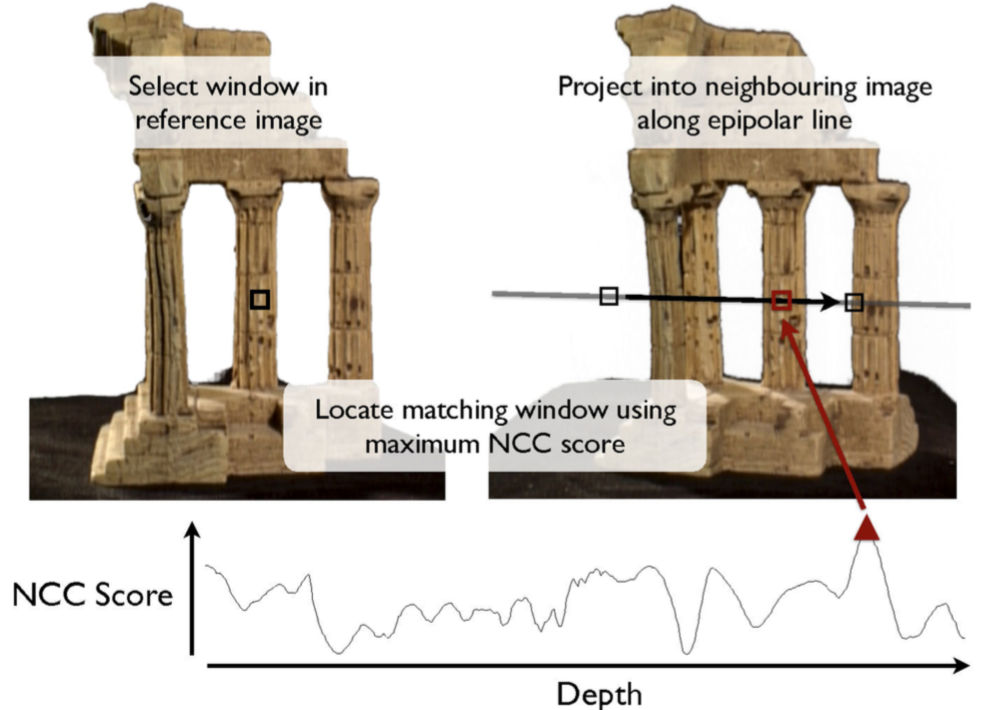
\includegraphics [width=0.7 \textwidth]{relatedwork/winner_takes_all}
\caption{Winner-takes-all strategy for depthmap reconstruction.}
\label{fig:winner_takes_all}\par % label should change \end{figure}
\end{figure}

In addition to the depth value with the highest photo-consistency score, the algorithm often evaluates a confidence measure so that low-confidence depth values can be ignored or down-weighted in the merging step \cite{hu2012quantitative}. This algorithm is first proposed in by \citeauthor{esteban2004silhouette}.

Though this simplistic approach can in general achieve good enough results, it's still problematic as occlusion or non-Lambertian effects might add noise to the photo-consistency score. Therefore, a larger window size is more likely leads to a stabler match. However, the associated peak will become broader and less well localized, reducing the accuracy of the depth estimate. \citeauthor{vogiatzis2007multiview} proposed a robust photo-consistency function to overcome this problem. The basic idea is that all potential causes of mismatches like occlusion, image noise, lack of texture, or highlights are treated as outliers. Matching is treated as a problem of robust model fitting to data containing outliers. More explicitly, for each pixel in the reference image, a photo-consistency curve $S_j(d)$ is computed for each visible view $j(j\in\mathcal{N}(i))$. Since simpling avering the photo-consistency scores across various views cannot handle outliers, they build a new $\mathcal{C}$ by detecting all the local maxima $d_k$ of $S_j$, and using a Parzen window with a kernel $W$ as follows:
\begin{equation}
\mathcal{C}(d) = \sum_{j\in\mathcal{N}(i)}\sum_k S_j(d_k)W(d - d_k)
\end{equation}\

This robust photo-consistency score can surpress local mixima, while simple averaging leads to erroneous results, see figure~\ref{fig:robust_pc}.

\begin{figure}[h]
\centering
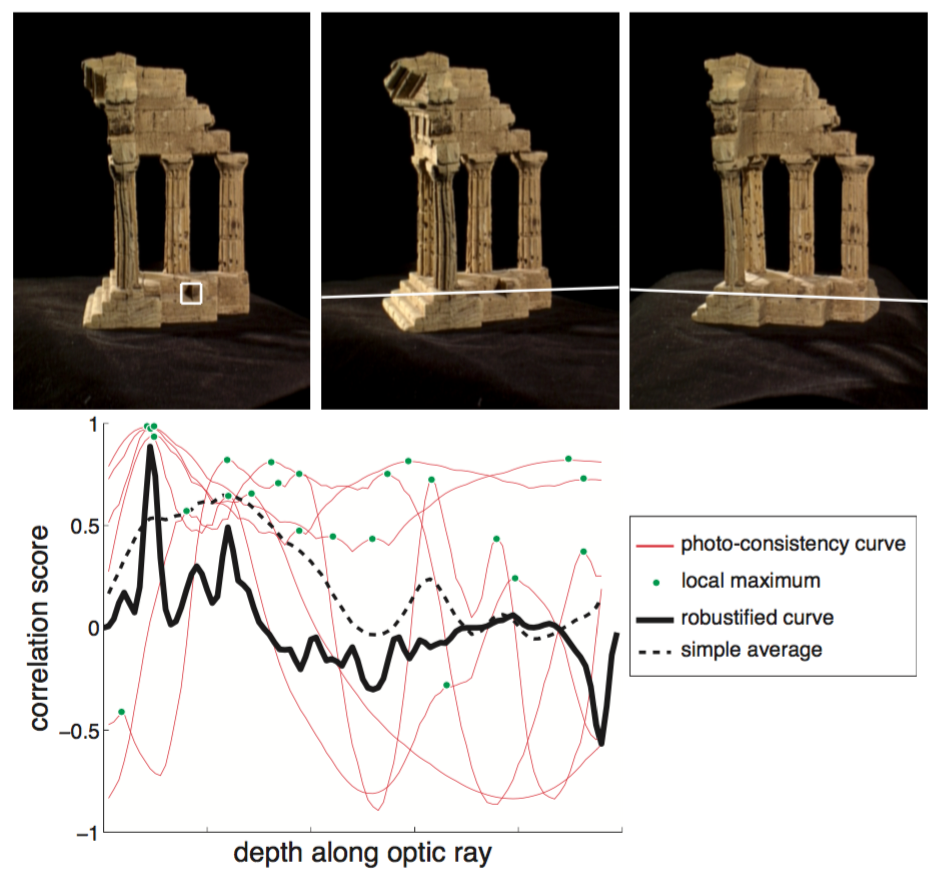
\includegraphics [width=0.7 \textwidth]{relatedwork/robust_pc}
\caption{Robust photo-consistency function by \citeauthor{vogiatzis2007multiview}}
\label{fig:robust_pc}\par % label should change \end{figure}
\end{figure}

\citeauthor{goesele2006multi} proposed a simpler yet effective approach, which is to compute the average of pairwise photo-consistency scores after ignoring those below a certain threshold.

\textbf{MRF Depthmaps} In the case of severe occlusion, there may not exist a correspondence in the other images. Spatial consistency can be enforced under the assumption that neighbouring pixels have similar depth values. This can be formulated under the Markov Random Field (MRF) framework, where the problem becomes minimizing the sum of a unary $\Phi(\cdot)$ and pairwise term $\Psi(\cdot, \cdot)$. The unary term is the cost of assigning a depth label $k_p$ from a label set to the pixel $p$, whereas the pairwise term is the cost of assigning depth label $k_p$, $k_q$ to a pair of neighbouring pixels $p$ and $q$, respectively.

\begin{equation}
E(k_p)= \sum_p \Phi(k_p) + \sum_{(p,q)\in\mathcal{N}}\Psi(k_p, k_q)
\end{equation}

The unary cost reflects the photo-consistency score, which in this case, is the inversely proportional to the photo-consistency score. The pairwise term enforces the spatial regularization, thus is proportional to the amount of depth discrepancy at neighbouring pixels. 

\subsubsection{Structured Light}

Structured light is considered one of the most accurate reconstruction technique. It is based on projecting a temporally or spatially modulated pattern onto the surface and viewing the illuminated surface from one or more points of view. The correspondence is easily detected from the projected and imaged pattern, which is triangulated to obtain the 3D point. Each pixel in the pattern is assigned a unique codeword, and the codeword is represented (change of word) by using grey level, colour or geometric representations. Structured light is classified based on the coding strategy: time-multiplex, neighbourhood codification and direct codification \cite{salvi2004pattern}. Time-multiplexing techniques generate the codeword by projecting a sequence of patterns. Neighbourhood codification represents the codewords in a unique pattern. Direct codification techniques define a codeword for every pixel, which is equal to its grey level or colour.

\textbf{Time-multiplexing} A sequence of patterns are successively projected onto the surface, the codeword for a given pixel is formed by the sequence of illuminaiton values for that pixel across the projected patterns. This kind of pattern can achieve high accuracy due to two factors: 1). the codeword basis is small, e.g., two for binary pattern, therefore, each bit is easily distinguishable; 2). a coarse-to-fine strategy is used, and the position of the pixel becomes more precise as the patterns are successively projected. We further classify these techniques as follows: 1). binary codeword; 2). $n$-ary codeword; 3). gray code combined with phase shifting; 4). hybrid techniques.

\textbf{Spatial Neighbourhood} This kind of technique concentrate all the coding in a unique pattern. The codeword that labels a certain pixel is obtained from a neighbourhood of the pixels around it. Normally, the visual features gathered in a neighbourhood are the intensity or colour of the pixels or groups of pixels around it.

\textbf{Direct codification} There are ways that can directly represent the codeword in each pixel. To achieve this, there is a need to use either a large range of colour values or introduce periodicity. However, this kind of pattern is highly sensitive to noise because the ``distance'' between codewords is nearly zero. Moreover, the perceived colour depends not only on the projected colour, but also the intrisic clour of the surface, therefore, reference images must be taken. This kind of coding can be classified as: 1). codification based on grey levels; 2). codification based on colour.

\subsection{Shading Cue}
The shading variations can reveal the surface normal orientation, which can be further integrated into a 2.5D height map. Shading variation depends on the shape (surface normal orientation), reflectance (material), and lighting (illumination), therefore is generally a ill-posed problem because difference shapes illuminated under different light conditions might produce the same image. This leads to a novel technique called Photometric Stereo in which surface orientaiton is determined from two or more images. The idea of Photometric Stereo is to vary the direction of the incident illumination between successive views while holding the viewing direction constant. This provides enough information to determine surface orientation at each pixel~\cite{woodham1979photometric}. This technique can produce a surface normal map with the same resolution of the input image, \ie to produce the pixel-wise surface normal map. Since the coefficients of the normal are continous, the integrated height map can reach an accuracy that cannot be achieve by any triangulation methods. Therefore, photometric stereo is more desirable if the intrisic geometric details are of great importance.

Despite the superior results achieved by Photometric Stereo,  traditional photometric stereo generally makes the following assumptions:
\begin{itemize}
\item Camera: orthographic projection, linear radiometric response
\item Reflectance: known reflectance properties, \eg Lambertian in \cite{woodham1980photometric}, specular in \cite{}.
\item Illumination: the lighting conditions are parallel rays with known directions and intensities.
\item Others: shadow, interreflection, and other global light transportation are neglected
\end{itemize}

The key problem is how to generalize the assumptions of photometric stereo. For the camera assumption, orthographic projection can be achieved by using a lens with long focus and placing the objects far from the camera. The nonlinear response can be solved by performing radiometric calibration. The shadow and other global light transportation are one of the sources of errors, some approaches consider them as outliers and remove them before normal estimation. The reflectance and lighting assumptions, however, are the most complicated ones since the reflectance properties depends on material property and the microscopic structure, and the lighting can have arbitray or fixed position, orientation, and intensity. Therefore the research on Photometric Stereo are generally on three directions: 1). traditional photometric stereo with known reflectance and lighting conditions; 2). generalization of reflectance; 3). generalization of lighting conditions

\textbf{Traditional case} The Photometric Stereo is first proposed in~\cite{woodham1980photometric}. In this work, the Lambertian model is used, which is constant, and independent to incident and emit light direction.

\textbf{Generalization of Reflectance}
refer to \cite{alldrin2008photometric}

\textit{Parametric reflectance model} The reflectance is characterized by Bidirectinoal Reflectance Distribution Function (BRDF). Most BRDFs are more complicated than the Lambertian since relative few objects are either ideal diffuse or perfectly specular. The BRDF of many surfaces can be approximated as a combination of a Lambertian component and a specular component. This reflectance model has motiva{}ted a line of research~\cite{barsky20034,coleman1982obtaining,nayar1990determining}. \citeauthor{coleman1982obtaining} and \citeauthor{barsky20034} who treat specular pixels as outliers, and \citeauthor{schluns1993photometric}, \citeauthor{sato1994temporal}, and \citeauthor{mallick2005beyond} who assume the color of the specular lobe differs from the color of the diffuse lobe, allowing separation of the specular and diffuse components.

\textit{Non-parametric reflectance model} While parametric reflectance models are very good at reducing the complexity of BRDFs, they are usually only vaid for a imited class of materials. An alternative is to exploit physical properties common to a large classes of BRDFs. Typical properties include energy conservation, non-negativity, Helmholtz reciprocity, isotropy, etc. Helmholtz stereopsis, introduced by \citeauthor{zickler2002helmholtz}, is on such technique, exploiting reciprocity to obtain surface reconstruction with no dependence to the BRDF. Isotropy is another physical property which holds for material without ``grain''. \citeauthor{tan2007isotropy} use both symmetry and reciprocity present in isotropic BRDFs to resolve the generalized bas-relief ambiguity. \citeauthor{alldrin2007toward} show that isotropy, with no further assumptions on surface shape or BRDF, can be utilized to recover the surface normal at each surface point up to a plane.

\textbf{Generalization of Lighting}

The generalized lighting condition is anything other than the the ideal case of using a single distant point light source in a dark room. Therefore, any general cases like natural ambient light, multiple point light sources with/without ambient lighting, etc. To make the problem more tractable, the reflectance model should no longer be a general one, otherwise, the problem would have too many degrees of freedom, which means many different shapes with an incorrectly estimated general reflectance, and an incorrectly estimated general lighting would generate the same image appearance with much higher probability.

[Some other papers to read] \\
- R. J. Woodham. Photometric method for determining sur-
face orientation from multiple images.\\
1. joint recovery of unknown shape and reflectance\\
- N. Alldrin, T. Zickler, and D. Kriegman. Photometric stereo with non-parametric and spatially-varying reflectance.\\
- D. Goldman, B. Curless, A. Hertzmann, and S. Seitz. Shape and spatially-varying BRDFs from photometric stereo.\\
- T. Higo, Y. Matsushita, and K. Ikeuchi. Consensus photometric stereo.\\
- B.Shi,P.Tan,Y.Matsushita,and K.Ikeuchi. Elevationangle from reflectance monotonicity: Photometric stereo for general isotropic reflectances.\\
- BOXIN SHI's PhD thesis\\
- Satoshi Ikehata's PhD thesis\\
2. a less restrained capture setup with arbitrary and unknown illumination\\
- H. Hayakawa. Photometric stereo under a light source with arbitrary motion\\
- T. Papadhimitri and P. Favaro. A new perspective on uncalibrated photometric stereo\\
- B. Shi, Y. Matsushita, Y. Wei, C. Xu, and P. Tan. Self-calibrating photometric stereo\\
3. combine both directions\\
- A.HertzmannandS.Seitz.Shapeandmaterialsbyexample: a photometric stereo approach.\\
- A. Hertzmann and S. Seitz. Example-based photometric stereo: shape reconstruction with general, varying BRDFs.\\
- W. M. Silver. Determining shape and reflectance using mul- tiple images. Master’s thesis, MIT, 1980.\\

% \subsection{Silhouette Cue}

% \subsection{Texture Cue}

% \subsection{Defocus Cue}

%%%%%%%%%%%%%%%%%%%%%%%%%%%%%%%%%%%%%%%%%%%%%%%%%%%%%%%%%%%%%%%%%%%%%%
\section{Visual Properties}
\label{sec:VisProp}

TBD





\endinput
